\subsection{Density Transformation and Conservation of Probability}

\begin{frame}
\slidesonly{
\begin{center}
	\huge \subsecname
\end{center}
}
\end{frame}

\subsubsection{Setting}

\begin{frame}%\frametitle{\subsubsecname}

\slidesonly{\underline{Setting}: }Let $X_1$ and $X_2$ be jointly continuous random variables with 
density function $f_{X_1, X_2}$:

\svspace{-3mm}

\begin{equation}
f_{X_1, X_2}(x_1, x_2) = f{(\vec x)} \qquad \vec x \in \Omega \subset \R^2
\end{equation}

\pause

and let $\vec g(\vec x) =\notesonly{ ( g_1(\vec x), g_2(\vec x))^\top =} ( g_1(x_1, x_2), g_2(x_1, x_2))^\top = (u_1, u_2)^\top = \vec u$ be a one-to-one mapping/transformation.

\svspace{-3mm}

\begin{center}
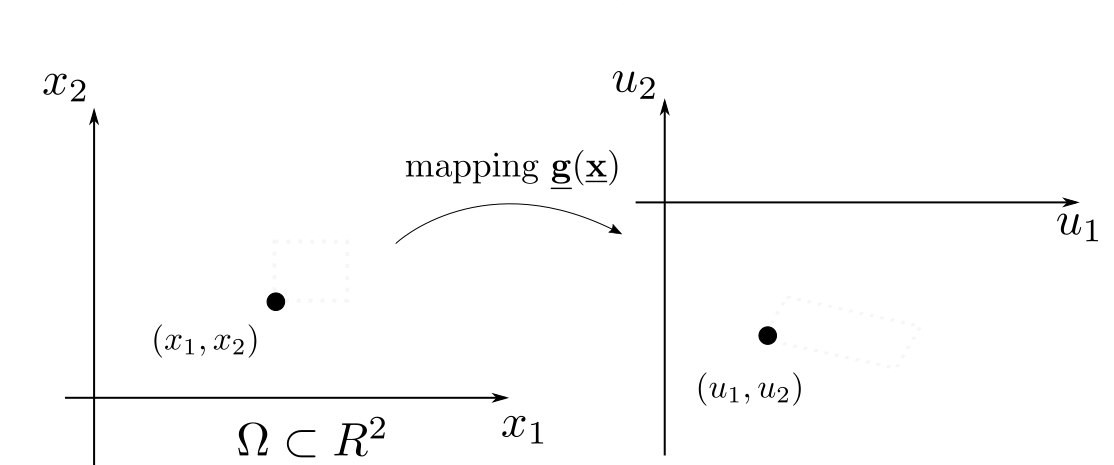
\includegraphics[width=0.7\textwidth]{img/xu_mapping}
\notesonly{\captionof{figure}{Transformation (mapping)}}
\end{center}

\svspace{-3mm}

\question{What requirement should this mapping fulfill?}

\pause

-conservation of probability.
\notesonly{The probability of the event $(x_1,x_2)$ should equal the probability of its counterpart in $(u_1,u_2)$ and vice-versa.}

\svspace{-8mm}

\begin{equation}
P_{\vec u}({\vec u}) \mathbf{d} {\vec u}
= \overbrace{P_{\vec x}({\vec x})}^{f (\vec {x})} \mathbf{d} {\vec x}
\end{equation}

\end{frame}

\begin{frame}{Conservation of probability}

\begin{center}
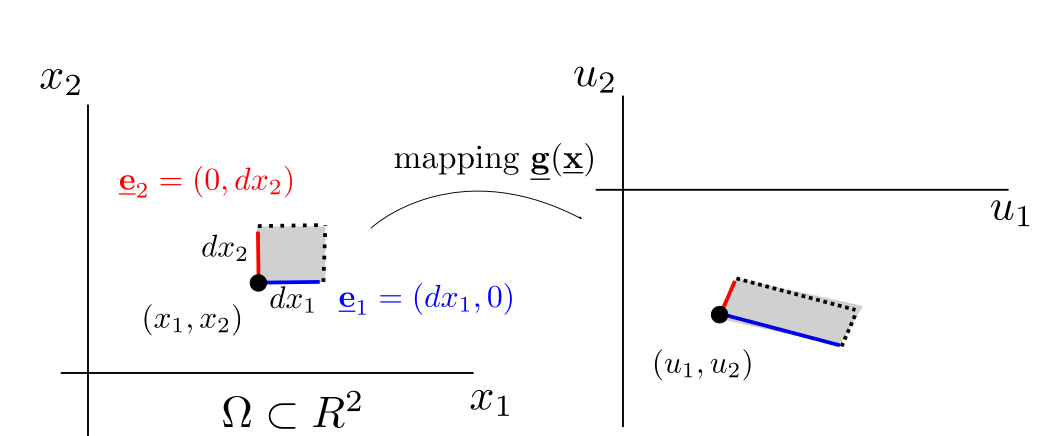
\includegraphics[width=0.7\textwidth]{img/u}
\notesonly{\captionof{figure}{Conservation of probability}}
\end{center}

The area of the small rectangle in $\Omega$ is $A = dx_1\, dx_2$.\\

\end{frame}


\begin{frame}{Conservation of probability}

\begin{center}
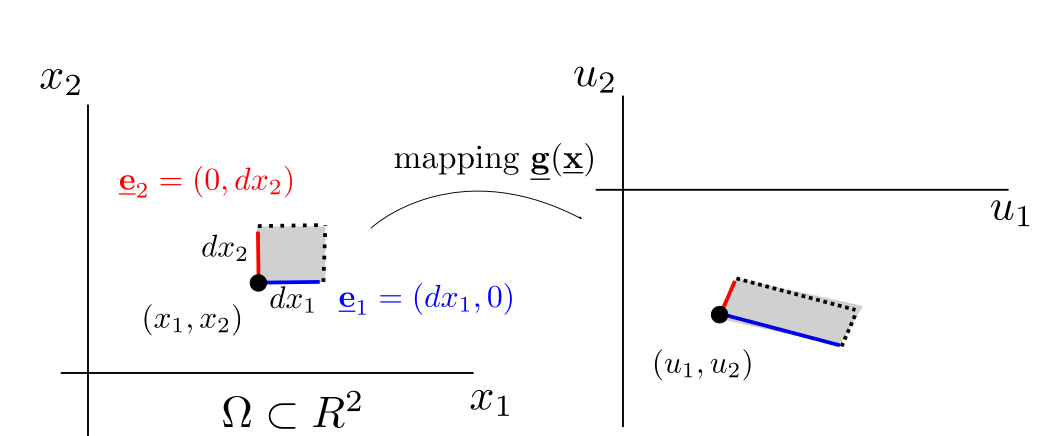
\includegraphics[width=0.7\textwidth]{img/u}
\notesonly{\captionof{figure}{Conservation of probability}}
\end{center}

The area of the small rectangle in $\Omega$ is $A = dx_1\, dx_2$\notesonly{.\\
The goal is to show that in order for probability to be conserved}, we need to know by how much the area will grow or shrink as we move between the spaces and eventually compensate for this change.

\pause

This implies the following relationship which we will derive:
\begin{equation}
\int_{\Omega} f(\vec{x}) \mathbf{d}\vec{x}
=\int_{u(\Omega)} f(~\underbrace{\vec g^{-1}(\vec u)}_{= \vec x}~) \frac{1}{\left|\det \frac{\partial \vec{u}}{\partial \vec{x}} \right|} \mathbf{d}\vec{u},
\end{equation}

\notesonly{where $\vec g^{-1}(\vec u) = \vec x$ is the inverse mapping.}


\end{frame}

\begin{frame}{Conservation of probability}

\slidesonly{

\begin{center}
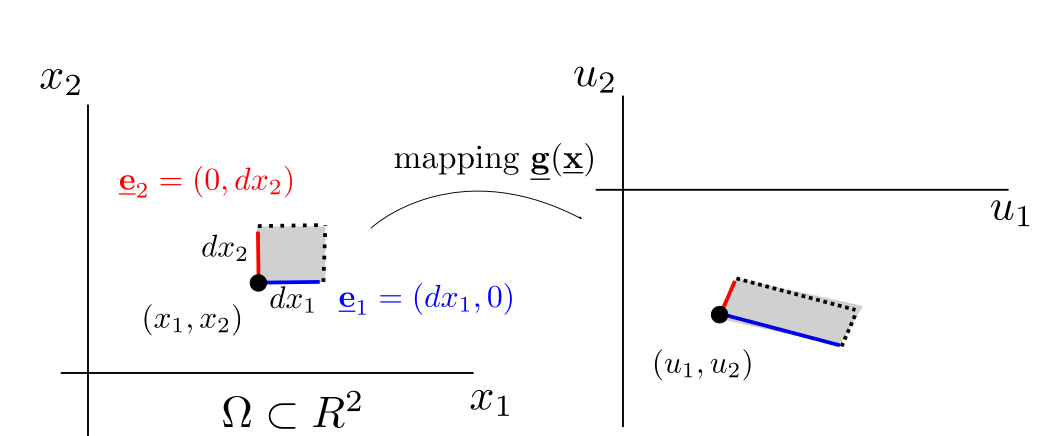
\includegraphics[width=0.7\textwidth]{img/u}
\notesonly{\captionof{figure}{Conservation of probability}}
\end{center}
}

\only<1>{

\begin{itemize}
\item Because $dx_1$ and $dx_2$ are \emph{infinitesimally small} we can consider the mapping from $\vec x$ to  
$\vec u$ to act as a \emph{linear} transformation, resulting in a different shape in $u(\Omega)$. 
\item The shape of the shaded area in $u(\Omega)$ is \emph{approximately} a parallelogram.
\item We will compute the ratio of the areas between the two transforms.
\item If we want to go back from $u(\Omega)$ to $\Omega$ we only need $\frac{1}{\text{ratio}}$.
\end{itemize}

}

\only<2>{


\underline{Important}:
Approximating the above as a linear transformation (i.e. a small rectangle turns into a parallelogram) only holds for very small $d\vec x$.


}

\only<3->{

Before we can compute the area of the parallelogram in $u(\Omega)$ we need to find out what the vectors ${\color{blue}\vec e_1}, {\color{red}\vec e_2}$ map to in $u(\Omega)$.

\question{How do we get the area of the parallelogram?}

}
\only<4>{

From vector calculus:
\notesonly{

The area of the parallelogram is the magnitude of the cross product between the two vectors.
}

\svspace{-3mm}

\begin{equation}
A_{\text{parr.}} = \big| \vec g({\color{blue}\vec e_1}) \times \vec g({\color{red}\vec e_2}) \big|
\end{equation}

}

\end{frame} 



\newpage

\subsubsection{Mapping the vectors}

\begin{frame}{\subsubsecname}

We first only consider the vector due to ${\color{blue}dx_1}$:

\svspace{-5mm}

\begin{center}
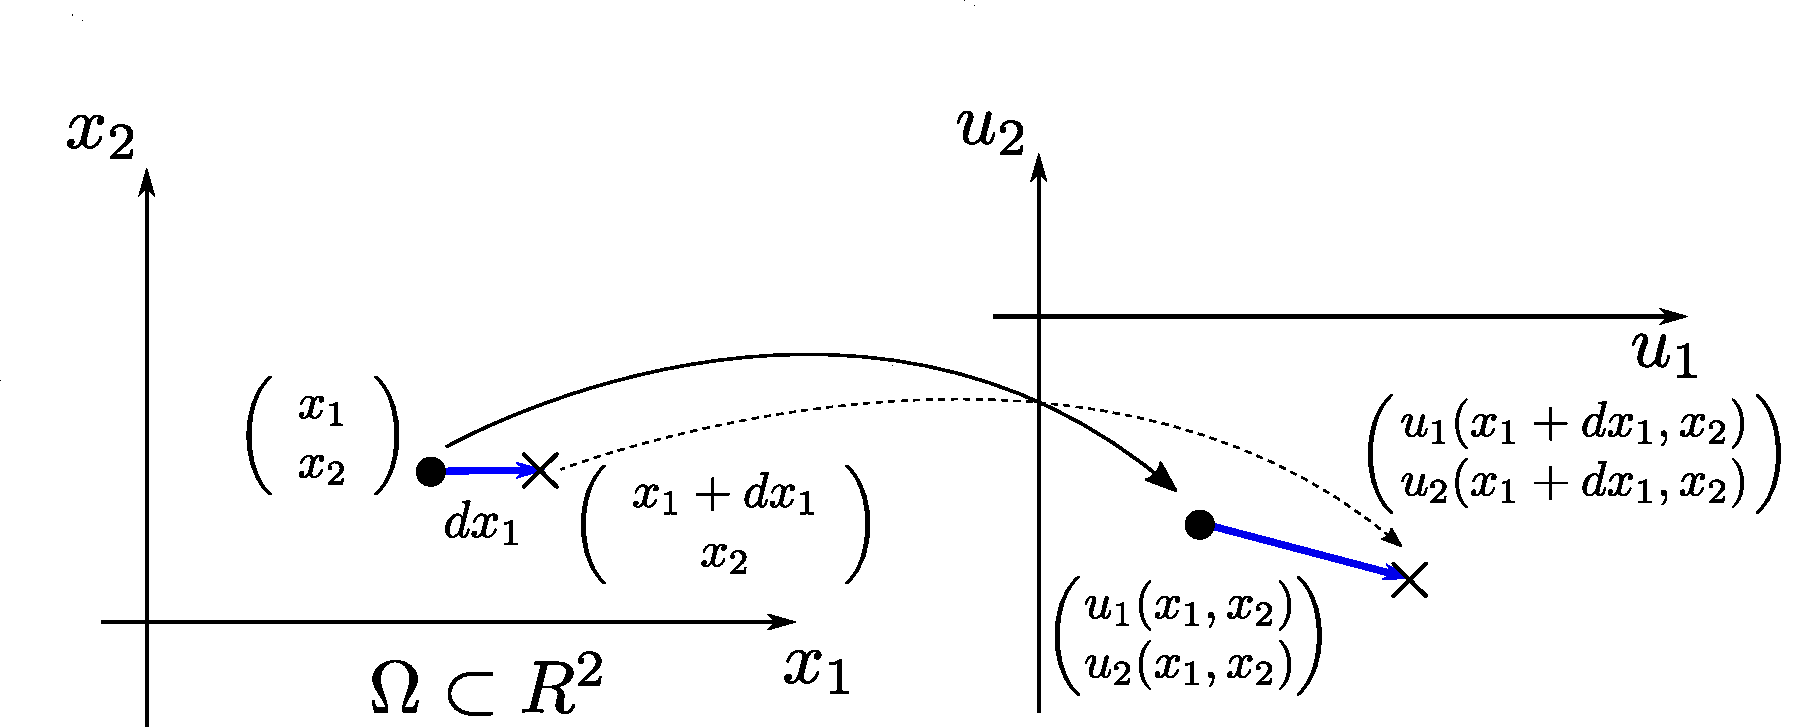
\includegraphics[width=0.75\textwidth]{img/x1.pdf}
\notesonly{\captionof{figure}{Mapping the first component}}
\end{center}

\svspace{-3mm}

\pause

The difference vector\notesonly{ between the two corresponding points} in $u(\Omega)$ becomes:

\begin{equation}
\begin{array}{r}
\rmat{
u_1 (x_1 + dx_1, x_2)\\
u_2 (x_1 + dx_{\color{magenta}1}, x_2)
} - 
\rmat{
u_1 (x_1, x_2)\\
u_2 (x_1, x_2)
} \\[0.7cm]
=
\rmat{
u_1 (x_1 + dx_1, x_2) - u_1 (x_1, x_2)\\
u_2 (x_1 + dx_{\color{magenta}1}, x_2) - u_2 (x_1, x_2)
}
\end{array}
\end{equation}

\end{frame}

\begin{frame}{\subsubsecname}

\slidesonly{
\svspace{-5mm}
\begin{center}
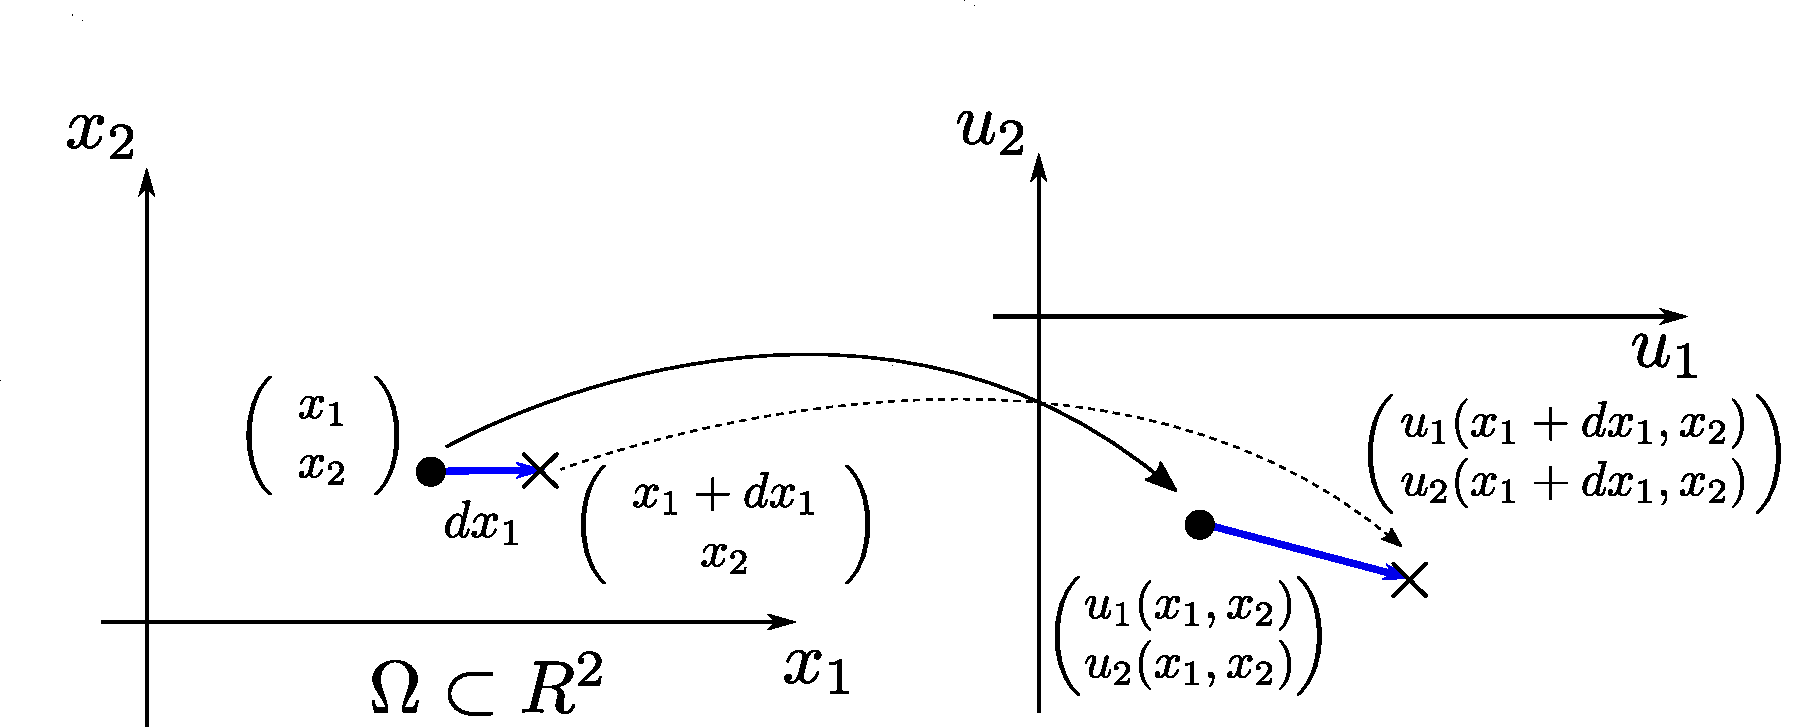
\includegraphics[width=0.75\textwidth]{img/x1.pdf}
\notesonly{\captionof{figure}{Mapping the first component}}
\end{center}

\svspace{-2mm}

\begin{equation}
\begin{array}{r}
\rmat{
u_1 (x_1 + dx_1, x_2) - u_1 (x_1, x_2)\\
u_2 (x_1 + dx_{\color{magenta}1}, x_2) - u_2 (x_1, x_2)
}
\end{array}
\end{equation}
}

\pause

Because $dx_1$ is so small, \only<4->{we can approximate the transformed vector by the derivative, 
which is essentially taking the limit $dx_1 \rightarrow 0$.\\
The difference vector in $u(\Omega)$ becomes:}

\only<3>{
\slidesonly{
\begin{center}

\includegraphics[width=0.2\textwidth]{img/meme_notthisagain}
\end{center}
}
}

\svspace{-3mm}

\only<5>{
\begin{equation}
\vec g: {\color{blue}\vec e_1} \mapsto 
\rmat{
\frac{\partial u_1}{\partial x_1} \Delta x_1\\[0.2cm]
\frac{\partial u_2}{\partial x_1} \Delta x_1
}
\end{equation}
}

\end{frame}

\begin{frame}{\subsubsecname}

\slidesonly{
\begin{center}
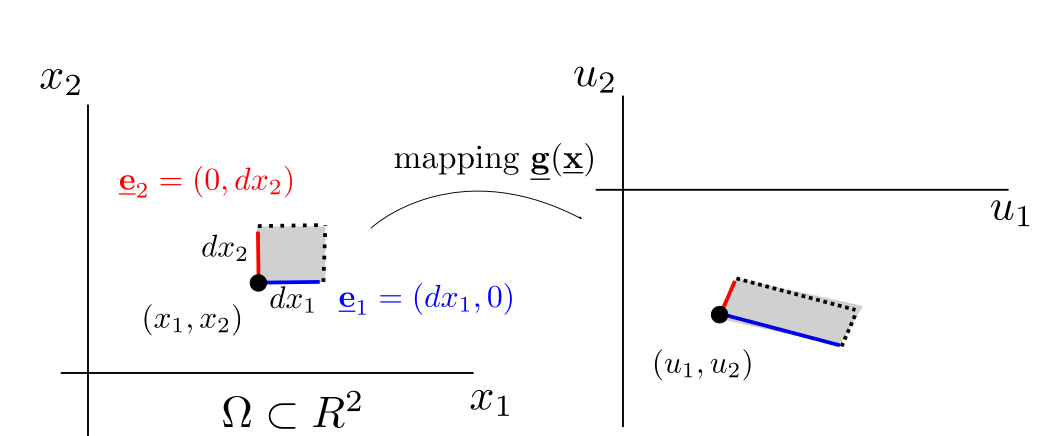
\includegraphics[width=0.6\textwidth]{img/u}
\end{center}
}

\question{What about ${\color{red}dx_2}$?}

\pause

- We use the same procedure on ${\color{red}\vec e_2}$:

\begin{equation}
u: {\color{red}\vec e_2} \mapsto 
\rmat{
\frac{\partial u_1}{\partial x_2} \Delta x_2\\[0.2cm]
\frac{\partial u_2}{\partial x_2} \Delta x_2
}
\end{equation}

\end{frame}

\begin{frame}{Computing the area of the parallelogram}

\svspace{-5mm}

\slidesonly{
\begin{center}
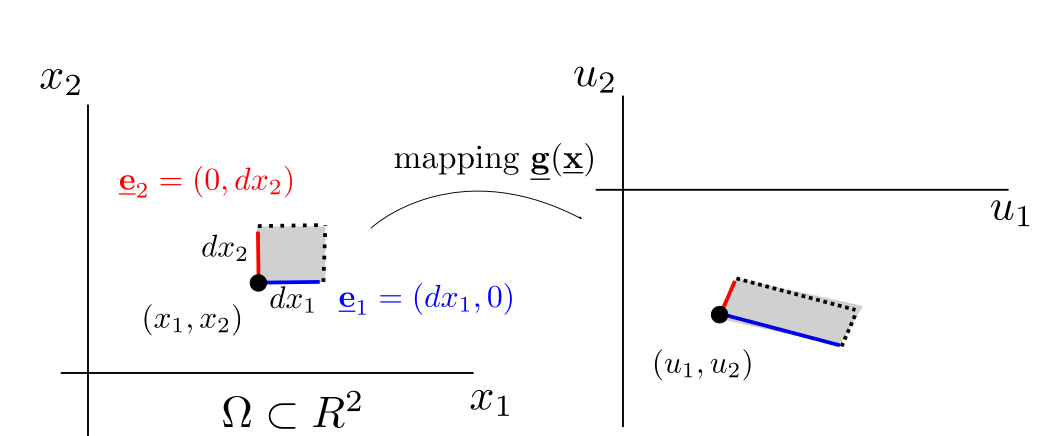
\includegraphics[width=0.6\textwidth]{img/u}
\end{center}
}

\slidesonly{

\svspace{-5mm}

\begin{center}
$$
u: {\color{blue}\vec e_1} \mapsto 
\rmat{
\frac{\partial u_1}{\partial x_1} \Delta x_1\\[0.2cm]
\frac{\partial u_2}{\partial x_1} \Delta x_1
}
\qquad\qquad
u: {\color{red}\vec e_2} \mapsto 
\rmat{
\frac{\partial u_1}{\partial x_2} \Delta x_2\\[0.2cm]
\frac{\partial u_2}{\partial x_2} \Delta x_2
}
$$
\end{center}

}

The area of the parallelogram spanned by the two difference vectors in $u(\Omega)$ 
is the magnitude of their cross product:
\slidesonly{
$$
A_{\text{parr.}} = \left| \; 
\rmat{
\frac{\partial u_1}{\partial x_1} \Delta x_1\\[0.2cm]
\frac{\partial u_2}{\partial x_1} \Delta x_1
}
\times
\rmat{
\frac{\partial u_1}{\partial x_2} \Delta x_2\\[0.2cm]
\frac{\partial u_2}{\partial x_2} \Delta x_2
}
\; \right|
$$
}

\end{frame}

\begin{frame}{Computing the area of the parallelogram}

\svspace{-3mm}

\begin{align}
A_{\text{parr.}} &= \left| \; 
\rmat{
\frac{\partial u_1}{\partial x_1} \Delta x_1\\[0.2cm]
\frac{\partial u_2}{\partial x_1} \Delta x_1
}
\times
\rmat{
\frac{\partial u_1}{\partial x_2} \Delta x_2\\[0.2cm]
\frac{\partial u_2}{\partial x_2} \Delta x_2
}
\; \right|\\ 
&=
\left| \; 
\underbrace{
\frac{\partial u_1}{\partial x_1} \frac{\partial u_2}{\partial x_2}
\; - \;
\frac{\partial u_1}{\partial x_2} \frac{\partial u_2}{\partial x_1}
}_{\text{the Jacobian determinant}}
\; \right| \Delta x_1 \Delta x_2 \\
&= 
\left| \; \det\,
\underbrace{
\left(
\frac{\partial (u_1, u_2)}{\partial (x_1,x_2)}
\right)
}_{\text{the Jacobian}}
\; \right| \, \underbrace{\Delta x_1 \Delta x_2}_{\substack{\text{Original area}\\ \text{in }\Omega}}
\end{align}

\end{frame}


\begin{frame}{The Jacobian}

\svspace{-3mm}

\slidesonly{
$$
\begingroup
\footnotesize
\underbrace{
A_{\text{parr.}} }_{\text{in }u(\Omega)}= 
\bigg| \; \det\,
\underbrace{
\left(
\frac{\partial (u_1, u_2)}{\partial (x_1,x_2)}
\right)
}_{\text{the Jacobian}}
\; \bigg| \, \underbrace{\Delta x_1 \Delta x_2}_{\substack{\text{Original area}\\ \text{in }\Omega}}
\endgroup
$$
}

\only<1>{
This matrix of partial derivatives is called the \emph{Jacobian}:
\begin{equation}
\frac{\partial (u_1, u_2)}{\partial (x_1,x_2)} = 
\frac{\partial (g_1(\vec x), g_2(\vec x))}{\partial (x_1,x_2)} = 
\frac{\partial \vec u}{\partial \vec x} =
\underbrace{
\rmat{
{\partial u_1}/{\partial x_1} & {\partial u_1}/{\partial x_2}\\[0.2cm]
{\partial u_2}/{\partial x_1} & {\partial u_2}/{\partial x_2}
}%rmat
}_{
\substack{
\text{matrix of}\\
\text{partial derivatives}
}%substack
}
\end{equation}
}

\end{frame}

\begin{frame}{Conservation of Probability}

\svspace{-3mm}

\slidesonly{
$$
\begingroup
\footnotesize
\underbrace{
A_{\text{parr.}} }_{\text{in }u(\Omega)}= 
\bigg| \; \det\,
\underbrace{
\left(
\frac{\partial (u_1, u_2)}{\partial (x_1,x_2)}
\right)
}_{\text{the Jacobian}}
\; \bigg| \, \underbrace{\Delta x_1 \Delta x_2}_{\substack{\text{Original area}\\ \text{in }\Omega}}
\endgroup
$$
}
\svspace{-3mm}

\question{What is the takeaway from this?}

\slidesonly{
\svspace{-5mm}

\begin{center}
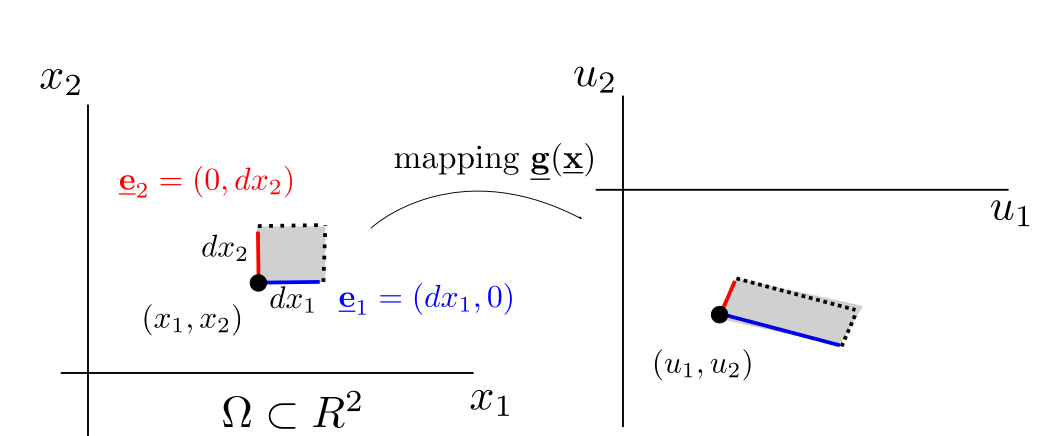
\includegraphics[width=0.55\textwidth]{img/u}
\end{center}
}

\pause

-\notesonly{If we are }given an area in $N$-dim space $\Omega$ spanned by $N$ small vectors ${\color{blue}\vec e_1}$, ${\color{red}\vec e_2},\ldots,\vec e_N$,
\notesonly{we can compute the area of the corresponding parallelogram in $u(\Omega)$ 
by multiplying the original area by the Jacobian determinant, i.e.
}

\svspace{-5mm}

\begin{equation}
A_{\text{parr.} \text{in }u(\Omega)}  = 
\Big| \; \det\, \overbrace{\text{Jacobian}}^{N \times N}
\; \Big| \, A_{\text{in }\Omega}
\end{equation}

\end{frame}

\subsubsection{Inverse mapping}

\begin{frame}{Conservation of probability}

\svspace{-3mm}

\slidesonly{
$$
\begingroup
\footnotesize
\underbrace{
A_{\text{parr.}} }_{\text{in }u(\Omega)}= 
\bigg| \; \det\,
\underbrace{
\left(
\frac{\partial (u_1, u_2)}{\partial (x_1,x_2)}
\right)
}_{\text{the Jacobian}}
\; \bigg| \, \underbrace{\Delta x_1 \Delta x_2}_{\substack{\text{Original area}\\ \text{in }\Omega}}
\endgroup
$$
}

\svspace{-3mm}


\question{What if we want to transform from $u(\Omega)$ back to $\Omega$?}


\only<1>{
\slidesonly{
\begin{center}

\includegraphics[width=0.5\textwidth]{img/meme_goback}
\end{center}
}
}

\pause

\svspace{-7mm}

\begin{center}
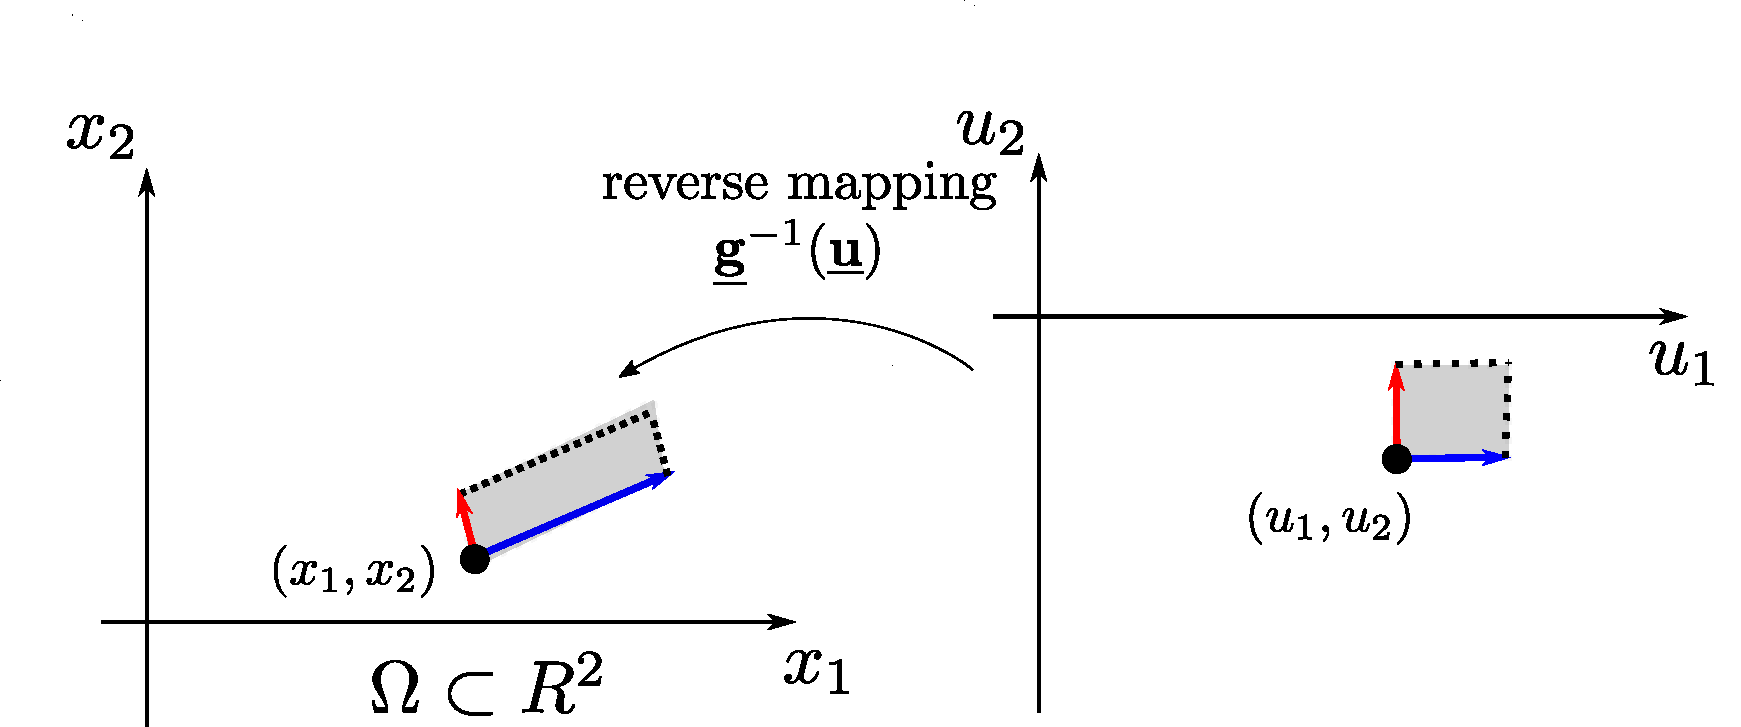
\includegraphics[width=0.6\textwidth]{img/reverse.pdf}
\notesonly{\captionof{figure}{Inverse mapping}}
\end{center}

We apply the inverse mapping $\vec g^{-1}(\vec x)$\notesonly{, assuming it exists and is differentiable. A very small rectangle in $u(\Omega)$ transforms into a parallelogram in $\Omega$.} 
This reverse transformation would require the inverse of the above matrix of partial derivatives.
\notesonly{The matrix of partial derivatives tells us how to transform infinitesimally small vectors back and forth.}

%Transformation between the spaces for infinitesimally small vectors:

%$$
%\rmat{
%u_1(x_1) & u_1(x_2)\\
%u_2(x_1) & u_2(x_2)
%}
%\rmat{
%a\\
%b
%}
%=
%\rmat{
%u_1(x_1)\\
%u_2(x_1)
%}
%a
%+
%\rmat{
%u_1(x_2)\\
%u_2(x_2)
%}
%b
%$$

\end{frame}

\begin{frame}{\subsubsecname}

\slidesonly{
$$
\begingroup
\footnotesize
\underbrace{
A_{\text{parr.}} }_{\text{in }u(\Omega)}= 
\bigg| \; \det\,
\underbrace{
\left(
\frac{\partial (u_1, u_2)}{\partial (x_1,x_2)}
\right)
}_{\text{the Jacobian}}
\; \bigg| \, \underbrace{\Delta x_1 \Delta x_2}_{\substack{\text{Original area}\\ \text{in }\Omega}}
\endgroup
$$

$$
\begingroup
\footnotesize
\underbrace{
A_{\text{parr.}} }_{\text{in }\Omega}=\ldots
\endgroup
$$
}


\question{Do we really have to compute the inverse of the matrix?}

\pause

- No, the determinant of the inverse matrix is 1 / det of the original matrix:
\begin{equation}
\frac{1}{\left| \det \left( \frac{\partial \vec u}{\partial \vec x} \right) \right|} =
{\left| \det \left( \frac{\partial \vec x}{\partial \vec u} \right) \right|}
\end{equation}

\end{frame}

\begin{frame}{Summary}

\underline{Transformation between probability densities:}

\notesonly{A transformation has to conserve the probabilities of events. }If the area represents the probability of the event, 
transforming it into another space should not \notesonly{cause any }increase or decrease \notesonly{in }the probability of the event.

Therefore, if we multiply the area of the rectangle in $\Omega$ by the pdf $f(\vec x)$ at $\vec x$, we get the probability of the parallelogram in $u(\Omega)$:

\begin{align}
\int_{\Omega} f(\vec{x}) \mathbf{d}\vec{x}
&=\int_{u(\Omega)} f(~\overbrace{{\vec g^{-1}(\vec u)}}^{= \vec x}~) \left|\det \frac{\partial \vec{x}}{\partial \vec{u}} \right| \mathbf{d}\vec{u}\\
&=\int_{u(\Omega)} f({\vec g^{-1}(\vec u)}) \frac{1}{\left|\det \frac{\partial \vec{u}}{\partial \vec{x}} \right|} \mathbf{d}\vec{u},
\end{align}

where $\vec g:\vec x \mapsto \vec g(\vec x)$ is a mapping \notesonly{with which we change the variables}\slidesonly{from} $\vec x$ to\notesonly{ a new coordinate system with coordinates} $\vec{u}=(g_1({\vec{x}}),\dots,g_N(\vec{x}))=(u_1,\dots,u_N)^{\top},$ whose inverse mapping
 $\vec g^{-1}(\vec{u})=\vec x$ exists and is differentiable.

\end{frame}

